\subsection{Projektstruktur}
Zunächst müssen die Daten in Java durch eine Datenstruktur abgebildet waren. Ich habe mich entschieden, allgemeine Eigenschaften eines Datums in einer abstrakten Oberklasse und spezifischen Unterklassen für die jeweiligen Kalendersysteme abzubilden. Hier ein UML-Diagramm:
\begin{figure}[h]
	\centering
	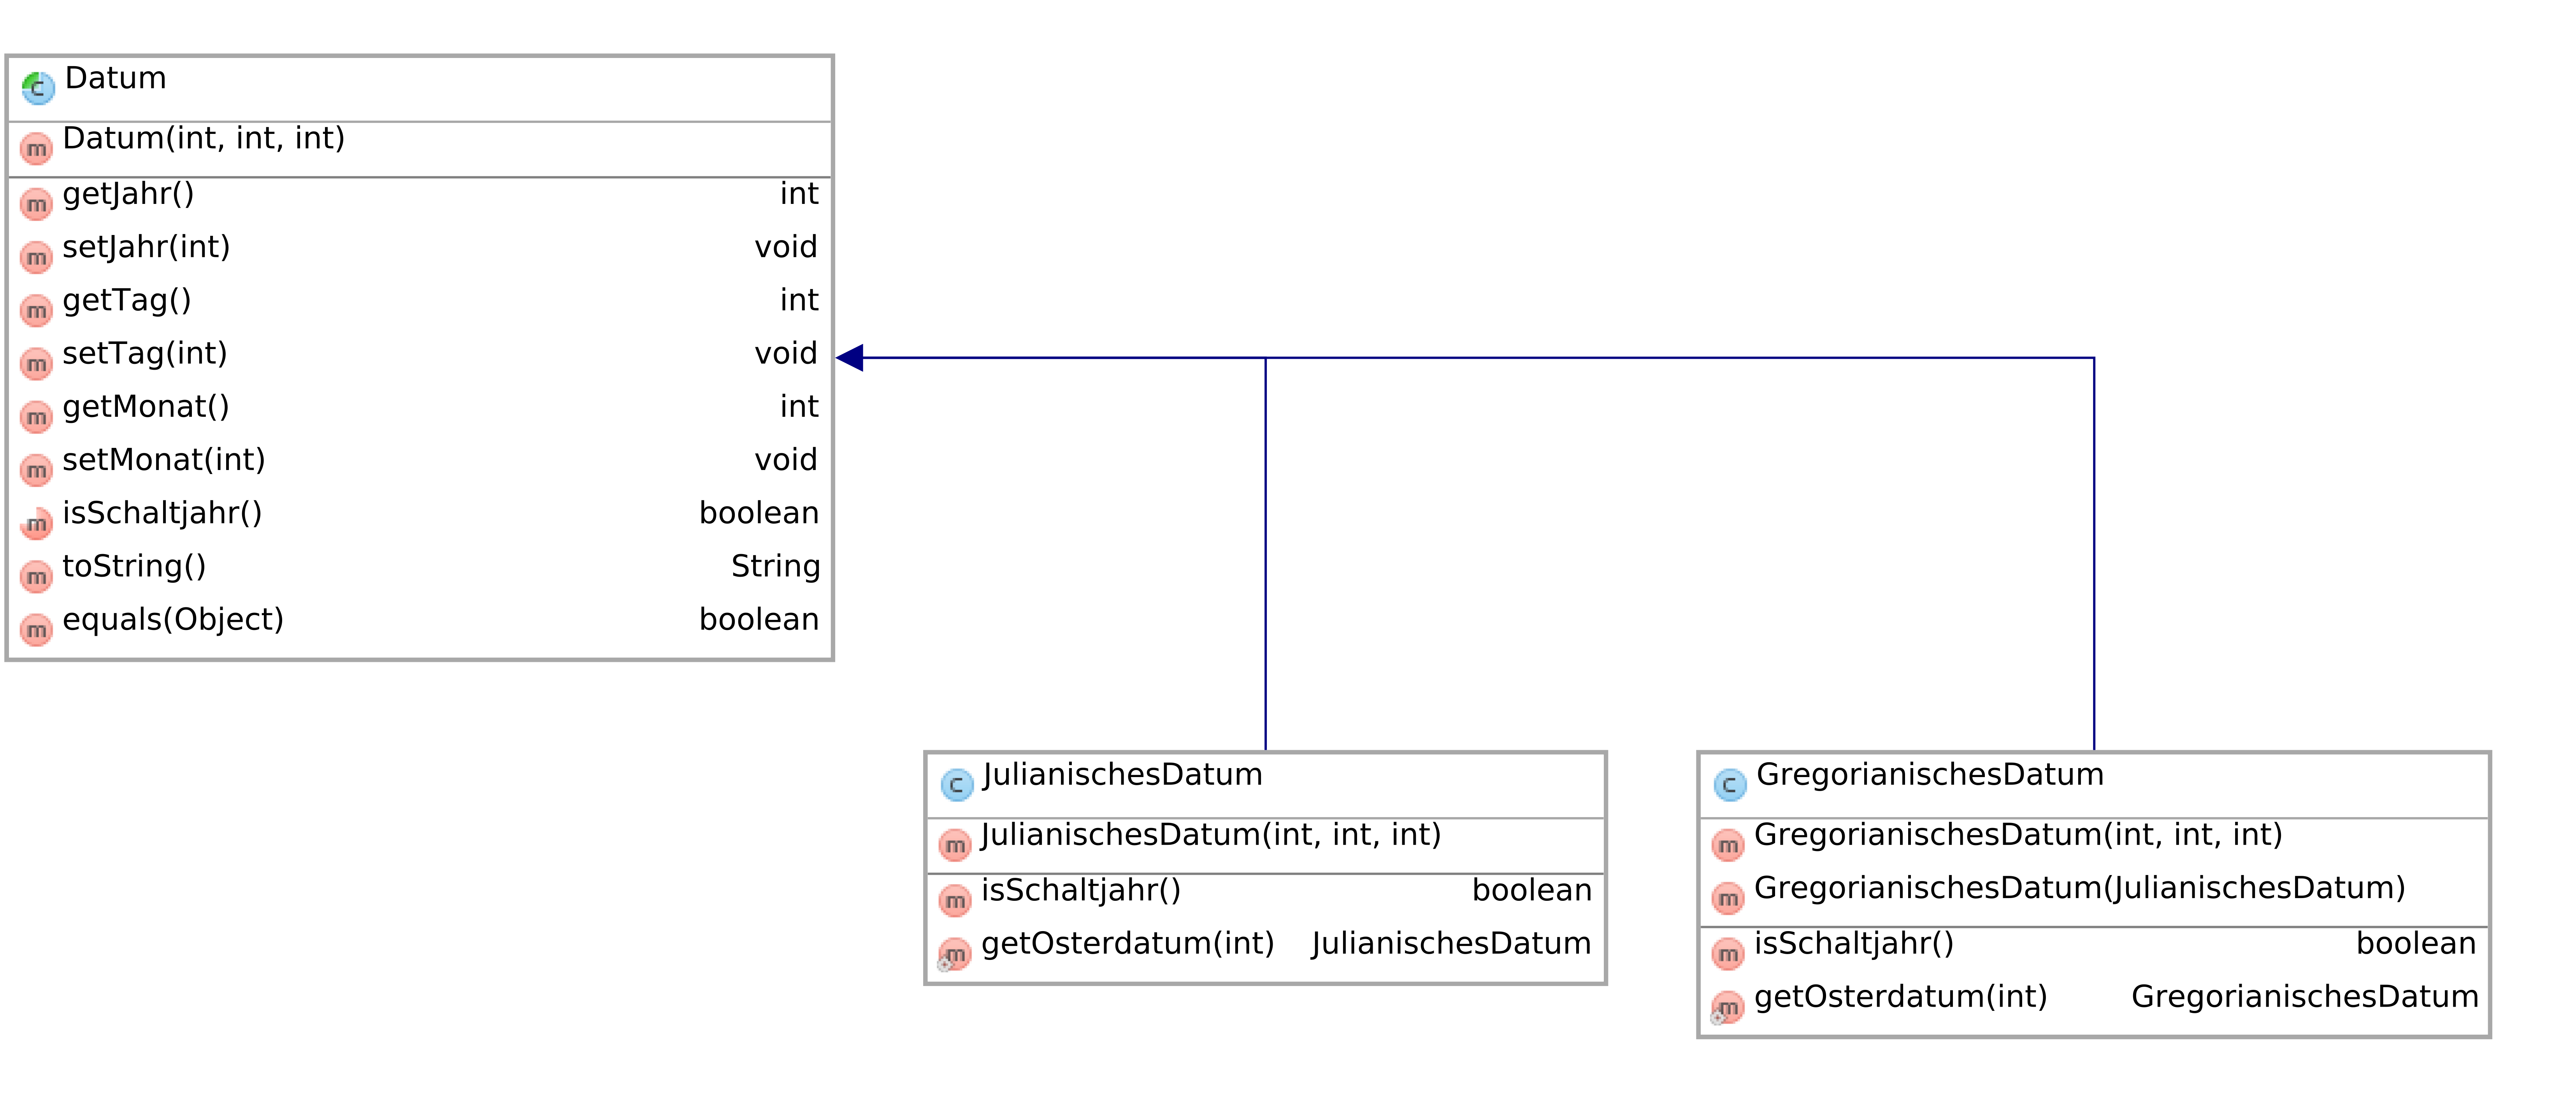
\includegraphics[width=\textwidth]{uml}
	\caption{UML-Diagramm der Implementation}
\end{figure}

Um beide Aufgabenstellungen bearbeiten zu können, muss nun für beide Kalnendersysteme getrennt die Osterformel implementiert werden. Da die Ausgabe im gregorianischen Kalendersystem gefordert wird und Daten verglichen werden, müssen Daten aus dem julianischen Kalender in den gregorianischen Kalender umgerechnet werden können. Dazu gibt es in der gregorianischen Klasse einen überladenen Konstruktor, der ein julianisches Datum entgegennimmt und wie im folgenden Kapitel beschrieben umrechnet.

\subsection{Suchcode}
Die Suche vergleicht mittels einer Schleife solange Oster- und Weihnachtsdaten, bis diese sich gleichen.
\clearpage
\subsection{Implementierungen der beiden Kalendersysteme}
	\subsubsection{Implementierung des julianischen Datums}
	Das Schaltjahrkriterium des juliansichen Kalenders lässt sich als folgender boolescher Ausdruck formulieren:
	\begin{lstlisting}
	return getJahr () % 4 == 0;
	\end{lstlisting}
	\subsubsection{Implementierung des gregorianischen Datums}
	Auch hier habe ich das Schaltjahkriterium als booleschen Ausdruck formuliert:
	\begin{lstlisting}
	return ( getJahr () % 4 == 0 && getJahr () % 100 != 0) || ( getJahr () % 400 ==0) ;
	\end{lstlisting}
	Außerdem gibt es in dieser Klasse eine Umrechnungsfunktion von dem julianischen in den gregorianischen Kalender. 

	Zunächst wird dabei das julianischem Datum in die entsprechenden Felder übernommen. Danach wird mit der in der Lösungsidee genannten Formel der Abstand zwischen den beiden Kalendersystemen in dem Jahr des Datums berechnet. Dieser Abstand wird dem Tag hinzuaddiert. 

	Danach wird die Funktion korrigiereUeberhang() aufgerufen. Diese ermittelt zünachst die für das Jahr des Datums zutreffenden Monatslängen (Schaltjahr). Falls durch das hinzuaddieren der Tagesdifferenz die Monatsläge überschritten wurde, korrigiert die Funktion das Datum folgenderemaßen:

	Zunächst wird berechnet, um wie viele Tage die Monatslänge überschritten wurde. Im folgenden wird diese Differenz als Überhang bezeichnet.

	Da die Tage die Monatslänge überschritten haben, muss das Datum mindestens im nächsten Monat liegen. Daher wird der Monat des Datums um eins erhöht. Ist der aktuelle Monat ein Dezember, wird dementsprechend das Jahr um 1 erhöht, der Monat auf Januar gesetzt und der Schaltjahresregel entsprechend die für das neue Jahr gültigen Monatslängen gesetzt.

	Unterschreiten oder gleichen die überhängenden Tage die Monatslänge des neuen Monates, ist die Umrechnung beendet. Die noch überhangenden Tage entsprechen dann dem Tag des neuen Monates.

	Überschreiten die überhägenden Tage die Monatslänge des neuen Monates, wird auch dieser Monat übersprungen. Außerdem wird der Überhang um die Monatslänge des übersprungenen Monats verringert, da ja der Monat übersprungen wurde.

	Dies wird solange wiederholt, bis das Datum erfolgreich umgerechnet wurde.